% TODO:
% --   domande età e primo approccio tecnologia, da vedere.
% --   da sistemare grafico età
% --   da sistemare grafico bravura pc (al posto di smartphone)
% --   cambiare titolo grafico età primo approccio tecnologia con:
%                "Età del primo approccio alla tecnologia"
% --   sistemare anche usi app spesa (colori)
% --   dati incrociati e correlazioni (Finire?)
Al fine di ottenere una corretta segmentazione demografica dei potenziali utenti dell'applicazione, si è effettuata
un'analisi etnografica.
Tale tipologia di analisi risulta necessaria per ottenere 
alcune informazioni fondamentali dagli utenti, di cui si terrà conto in seguito durante la fase di progettazione della UI e delle interazioni 
dell'applicazione. Al fine di ottenere informazioni sulla suddivisione demografica dei potenziali utenti, si è creato
un form anonimo tramite il software google forms\cite{GoogleModules}, che consente di creare, condividere ed analizzare in modo semplice
questionari di varia natura.

\subsection{Il sondaggio}
Il sondaggio proposto è composto da varie domande mirate alla
classificazione dei potenziali utenti rispetto ad alcune caratteristiche
fondamentali:
\begin{itemize}
	\item Età;
	\item sesso;
	\item relazione con la tecnologia;
	\item dispositivi con cui è stato effettuato il primo approccio alla tecnologia;
	\item competenze culinarie;
	\item esperienza o interesse rispetto alle applicazioni dedicate alla cucina o alla spesa.
\end{itemize}

Per raggiungere tale scopo sono state poste le seguenti semplici domande a
risposta multipla.

\subsubsection{Domande relative al profilo sociale degli utenti}
\begin{quote}
	\textbf{Sesso}
\end{quote}
La domanda posta permette di individuare la percentuale di partecipanti rispetto 
al sesso.  I risultati hanno rilevato un leggero vantaggio di utenti
di sesso femminile.

\begin{figure}[H]
	\centering
	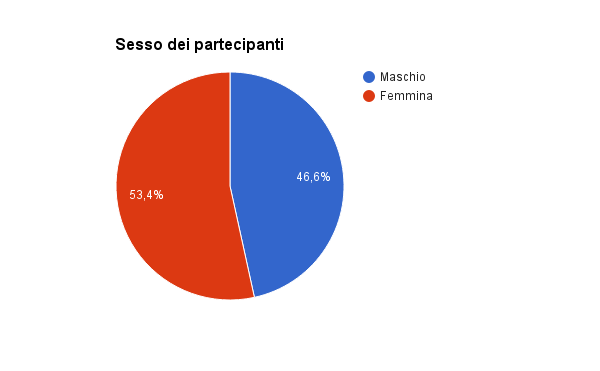
\includegraphics[scale=0.6]{img/chart_sesso}
\end{figure}

\begin{quote}
	\textbf{Età}
\end{quote}
AL fine di valutare l'età media dei potenziali utenti rispetto al primo approccio ai computer si sono individuate le seguenti fasce d'età:
\begin{itemize}
		\item Meno di 20 anni, ``nativi digitali", persone che si
			trovano a stretto contatto con i computer e gli
			smartphone moderni fin dai primi anni di vita.

		\item Da 20 a 30 anni, persone che hanno acquisito molta
			familiarità con i computer durante la propria infanzia o nella
			prima adolescenza.

		\item Da 30 a 40 anni, una parte di popolazione che ha avuto accesso
			a computer o altri calcolatori durante l'adolescenza o nei primi anni
			dell'età adulta.

		\item Da 40 a 50 anni, persone che hanno avuto in maggioranza il primo contatto con i device nei primi anni 
			della loro età lavorativa.

		\item Da 50 a 60 anni, persone la quale familiarità tecnologica è
			stata introdotta durante la loro professione.
			Presentano inoltre piccoli disturbi legati all'età.

		\item Più di 60 anni, ``pensionati digitali",  persone il quale rapporto con la
			tecnologia avviene solamente per cultura personale e con
			notevoli disturbi legati all'età.
\end{itemize}

Dai risultati possiamo evincere come i partecipanti al sondaggio siano per la maggior parte appartenenti alla fascia d'età compresa
fra 20 e 30 anni. Tale distribuzione demografica dipende certamente dai metodi utilizzati per diffondere il sondaggio, che è stato
condiviso via social network. Al fine di ridurre tale effetto, si sono contattati parenti di età diversa.

\begin{figure}[H]
	\centering
	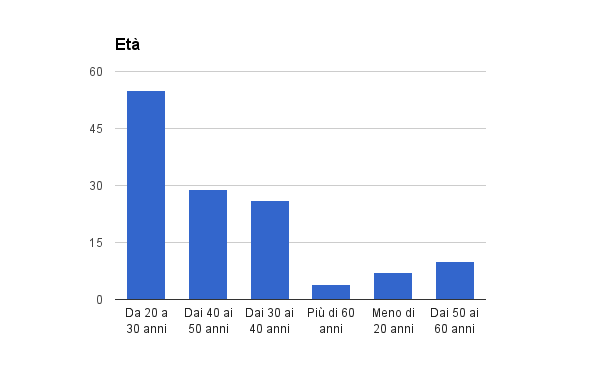
\includegraphics[scale=0.6]{img/chart_eta}
\end{figure}

\begin{quote}
	\textbf{Qual è il tuo livello di istruzione?}
\end{quote}
Tale domanda è utile per individuare il livello di istruzione degli utenti, un parametro che ha un impatto sulla interazione con l'applicazione.
I prerequisiti culturali necessari per utilizzare un'applicazione devono essere adeguati rispetto al livello medio di istruzione rilevato.
È facile infatti intuire come una applicazione dedicata all'alta cucina, che faccia ampio uso di termini in lingua francese, possa
risultare di difficile utilizzo per gli utenti meno istruiti.
Rispetto all'istruzione si sono individuati i seguenti titoli di studio:
\begin{itemize}
	\item Licenza elementare;
	\item licenza media;
	\item diploma di scuola superiore;
	\item laurea o superiore.
\end{itemize}
Data anche l'età media dei partecipanti al sondaggio, si è riscontrato uno squilibrio nei confronti del diploma di scuola superiore.

\begin{figure}[H]
	\centering
	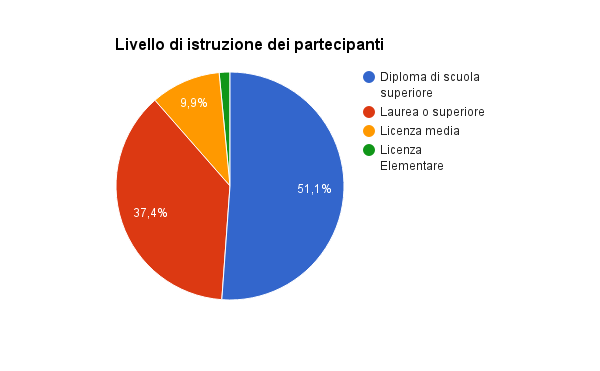
\includegraphics[scale=0.6]{img/chart_istruzione}
\end{figure}

\begin{quote}
	\textbf{Che lavoro fai?}
\end{quote}
La segmentazione degli utenti rispetto al loro impiego è una modalità non invasiva
per ottenere informazioni sulla classe sociale di appartenenza dei partecipanti.
Sebbene la classe sociale di appartenenza sia infatti un parametro molto interessante, ad esempio
per valutare il livello di accesso alla tecnologia disponibile, non è possibile ottenere
tale informazione dagli utenti senza introdurre bias o avversione nei confronti del sondaggio.
Al fine di ottenere una valutazione, seppur approssimativa, si sono individuate le seguenti categorie lavorative:

\begin{itemize}
	\item Studente;
	\item operaio;
	\item impiegato;
	\item libero professionista;
	\item imprenditore;
	\item pensionato o casalinga;
	\item disoccupato.
\end{itemize}

Il numero degli studenti e impiegati è equiparabile, risultano
invece meno rappresentate le altre categorie.

\begin{figure}[H]
	\centering
	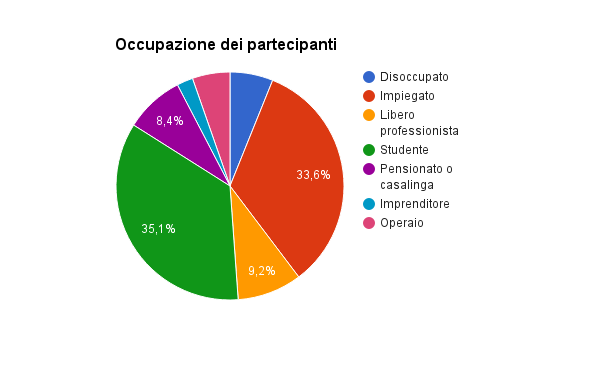
\includegraphics[scale=0.6]{img/chart_occupazione}
\end{figure}

\begin{quote}
	\textbf{Hai figli e/o nipoti? E se si, cucini per loro?}
\end{quote}

La presenza di un figlio implica la necessità di diversificare i piatti ed una
competenza di dominio più elevata rispetto alla media.\\

Dai grafici si deduce che la metà dei partecipanti possiede figli o nipoti, e
la maggior parte di essi cucina per i parenti.
\begin{figure}[H]
\centering
\begin{minipage}{.48\textwidth}
	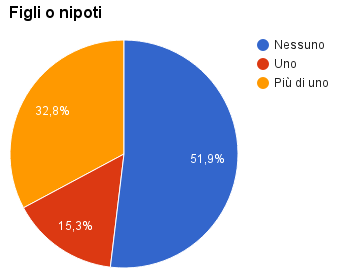
\includegraphics[scale=0.57]{img/chart_hai_figli_o_nipoti}
\end{minipage}
\hfill
\begin{minipage}{.49\textwidth}
	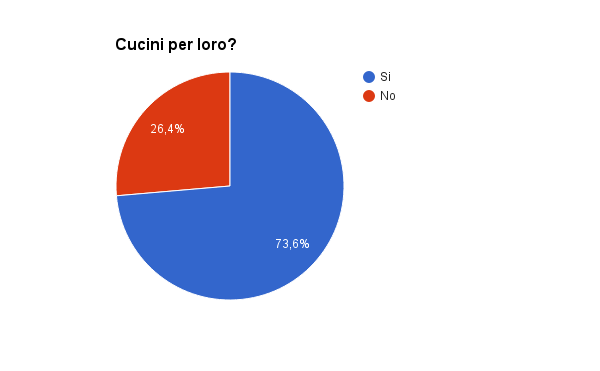
\includegraphics[scale=0.57]{img/chart_cucini_per_i_parenti}
\end{minipage}
\end{figure}

\subsubsection{Domande relative alle capacità tecnologiche degli utenti}
\begin{quote}
	\textbf{A che età hai avuto il primo approccio con la tecnologia?}
\end{quote}

Ricalcando la domanda posta per l'età del soggetto, vengono proposti i seguenti
scaglioni:

\begin{itemize}
	\item Fino a 6 anni;
	\item dai 6 ai 12 anni;
	\item dai 12 ai 20 anni;
	\item dai 20 ai 30 anni;
	\item dai 30 ai 50 anni;
	\item dopo i 50 anni.
\end{itemize}

Dal grafico si evince che la maggior parte degli utenti si è avvicinata alla
tecnologia durante la scuola dell'obbligo.

\begin{figure}[H]
	\centering
	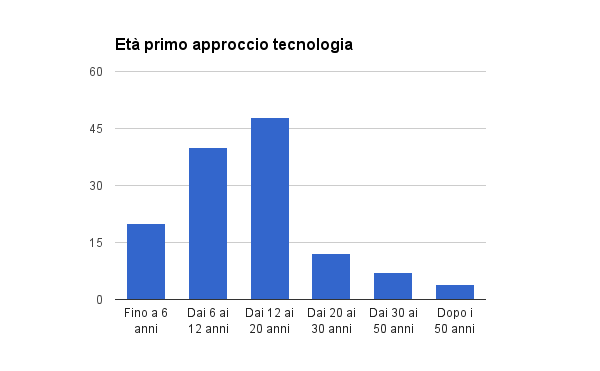
\includegraphics[scale=0.6]{img/chart_eta_primo_approccio}
\end{figure}

\begin{quote}
	\textbf{Con che genere di dispositivi?}
\end{quote}

Si è poi richiesto agli utenti di indicare quale fosse il primo calcolatore con il quale si è avuto
un contatto. Tale informazione fornisce un aiuto per individuare le competenze tecnologiche rispetto ai vari device.

\begin{itemize}
	\item Computer;
	\item smartphone;
	\item tablet;
	\item altro .
\end{itemize}

\begin{figure}[H]
	\centering
	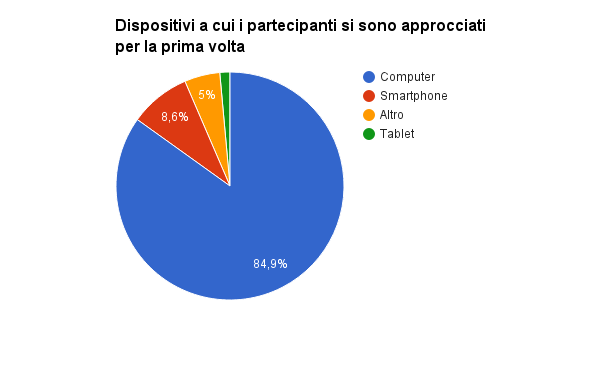
\includegraphics[scale=0.6]{img/chart_tipo_primo_approccio_dispositivi}
\end{figure}

\begin{quote}
	\textbf{Quanto ti ritieni competente con l'utilizzo di
	computer/smartphone?}
\end{quote}

Al fine di valutare la competenza tecnologica degli utenti con smartphone e computer, si è utilizzata
una scala compresa fra 1 e 5, dove 1 indica la competenza minima, 5 quella massima. Tale autovaltazione,
sebbene introduca certamente dei bias, risulta essere una misura interessante se non altro della competenza
percepita.
\\
È interessante notare come, in entrambe le valutazioni,
gli utenti si considerino su un livello medio-alto di competenza, con una maggioranza di valori pari a $3$ e $4$.
\begin{figure}[H]
\centering
\begin{minipage}{.48\textwidth}
	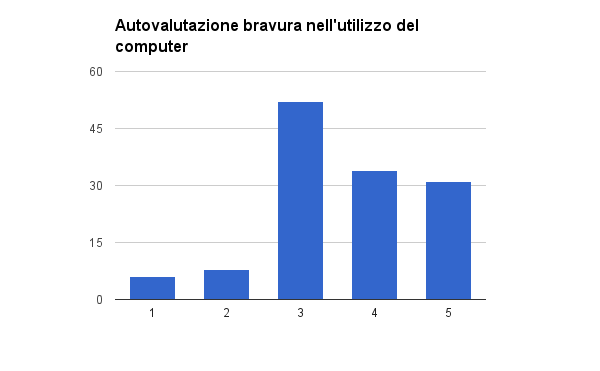
\includegraphics[scale=0.45]{img/chart_bravura_pc}
\end{minipage}
\hfill
\begin{minipage}{.49\textwidth}
	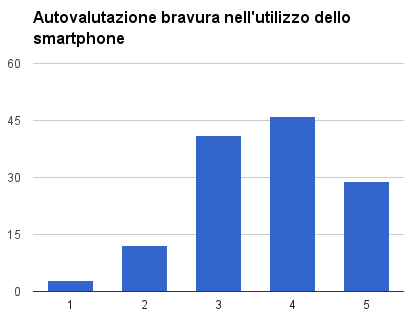
\includegraphics[scale=0.45]{img/chart_bravura_smartphone}
\end{minipage}
\end{figure}

\begin{quote}
	\textbf{Hai un problema al PC/telefono cellulare, che fai?}
\end{quote}

Al fine di valutare l'approccio degli utenti alla tecnologia, si è 
chiesto a questi ultimi come si comportino di fronte ai problemi con
i propri dispositivi. Le possibili risposte, in ordine decrescente di competenza da esse denotata, sono:
\begin{itemize}
 \item Cerco di risolvere da solo;
 \item Cerco di capire e localizzare il problema per dare più informazioni possibili all'assistenza ma non tocco niente;
 \item Chiamo l'assistenza o un amico;
 \item Lo butto e ne compro un altro.
\end{itemize}

La maggior parte degli utenti intervistati dimostra intraprendenza: più dei due terzi cercano almeno di comprendere
il problema da soli, mentre più della metà tenta addirittura di risolvere i problemi.

\begin{figure}[H]
	\centering
	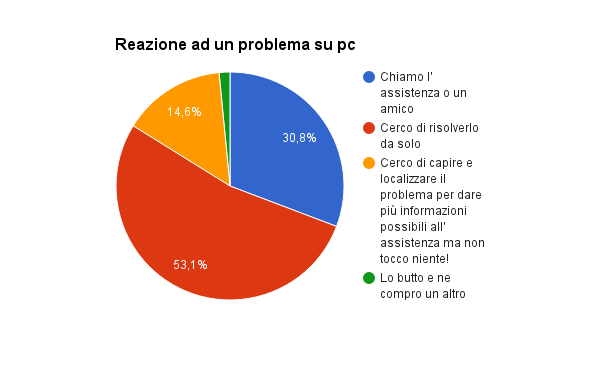
\includegraphics[scale=0.6]{img/chart_reazione_problema_pc}
\end{figure}

\subsubsection{Domande relative alla capacità culinaria}

\begin{quote}
	\textbf{Quanto ti ritieni competente in cucina?}
\end{quote}

Utilizzando una scala con valori fra 1 e 5 è stato chiesto agli utenti di valutare la propria competenza culinaria.
Tale informazione è utile a inquadrare gli utenti rispetto alla loro competenza specifica di dominio. Un cuoco esperto, infatti,
avrà di certo requisiti diversi rispetto a uno alle prime armi.
\\
La distribuzione delle autovalutazioni ricalca una distribuzione normale con media 3. Gli utenti si divido infatti in modo
pressoché uniforme fra utenti competenti e utenti che non sono abili in cucina.


\begin{figure}[H]
	\centering
	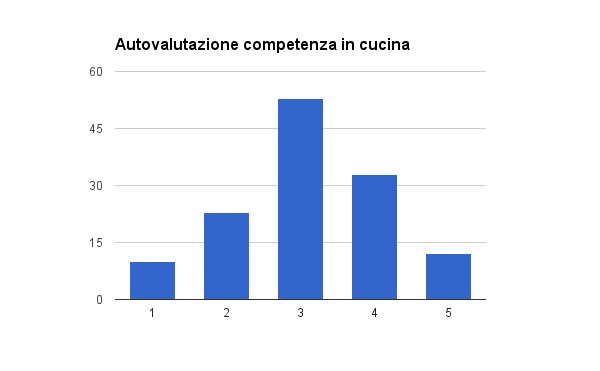
\includegraphics[scale=0.6]{img/chart_bravura_cucina}
\end{figure}

\begin{quote}
	\textbf{Degli amici si auto-invitano a casa tua per una cena, che fai?}
\end{quote}

Come nel caso della domanda precedente, anche in questo caso viene parzialmente misurata l'affinità degli utenti con la cucina.
Oltre a tale aspetto, si vuole comprendere quale sia l'approccio degli utenti all'improvvisazione culinaria, oltretutto
nel caso in cui si debba cucinare non solo per sé stessi. Le risposte possibili da noi previste sono le seguenti:
\begin{itemize}
 \item Inizio a sperimentare ai fornelli, voglio sorprendere tutti;
 \item Cerco qualche ricetta facile per stasera;
 \item Vado al supermercato per cercare qualcosa di semi pronto;
 \item Ordino qualcosa.
\end{itemize}

Dai risultati ottenuti la maggior parte (circa il 75\%) degli utenti è pronta a improvvisare una cena anche per i propri amici, mostrando
iniziativa e la volontà di cucinare per altri. Fra questi ultimi, la maggioranza cerca ricette facili, caso d'uso molto affine
ad un'applicazione di supporto alla cucina.

\begin{figure}[H]
	\centering
	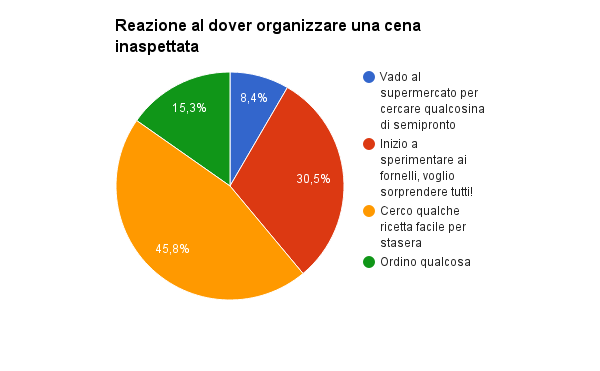
\includegraphics[scale=0.6]{img/chart_reazione_cena}
\end{figure}

\begin{quote}
	\textbf{Dove fai la spesa?}
\end{quote}
Il luogo o i luoghi nei quale viene effettuata la spesa da parte degli utenti. Tale informazione è doppiamente utile: da una parte,
è certamente correlata al ceto sociale di appartenenza, dall'altra, ci da informazioni sul livello di passione per il cibo del soggetto.
Le opzioni da noi previste sono:
\begin{itemize}
 \item Direttamente dal produttore al mercato;
 \item Ordino la spesa online;
 \item Piccoli commercianti;
 \item Supermercato.
\end{itemize}
Come era del resto prevedibile, la stragrande maggioranza degli utenti utilizzano i supermercati come fonti di cibo, mentre sono in minoranza quelli che
scelgono le altre opzioni. Questa informazione ci aiuta a comprendere come si possano aiutare gli utenti nell'effettuare la spesa.

\begin{figure}[H]
	\centering
	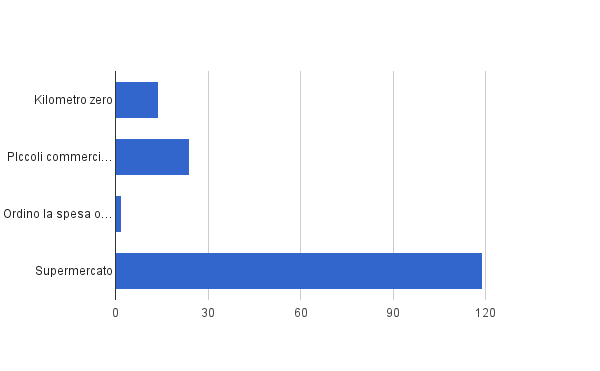
\includegraphics[scale=0.6]{img/chart_dove_fai_la_spesa}
\end{figure}

\begin{quote}
	\textbf{Hai allergie o intolleranze al cibo?}
\end{quote}

Con questa domanda si intende valutare l'impatto di allergie varie sulla popolazione totale. Si è scelto inoltre di contare chi ha intolleranze multiple.
Dai risultati ottenuti emerge come l'impatto di allergie sulla popolazione sia minoritario ma non trascurabile.

\begin{figure}[H]
	\centering
	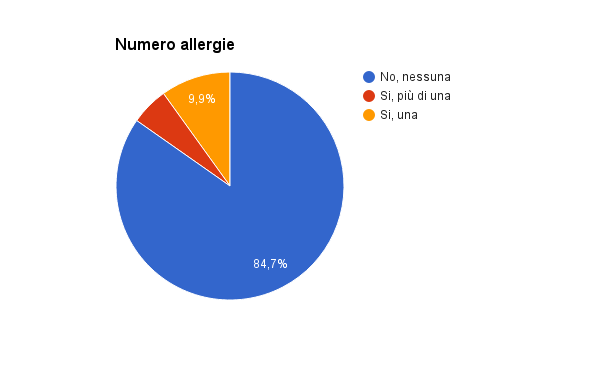
\includegraphics[scale=0.6]{img/chart_allergie}
\end{figure}

\begin{quote}
	\textbf{Usi app o siti web per cucinare? Se hai risposto no, ti interesserebbe un'app per cucinare?}
\end{quote}

Tramite tali domande si intende valutare da una parte la diffusione di software per l'ausilio alla cucina, dall'altra
l'interesse per un'eventuale applicazione fra chi non utilizza tali software. La maggior parte degli utenti utilizza un'applicazione,
chi non utilizza strumenti software è in gran parte interessato ad un'applicazione di questo tipo.

\begin{figure}[H]
\centering
\begin{minipage}{.48\textwidth}
	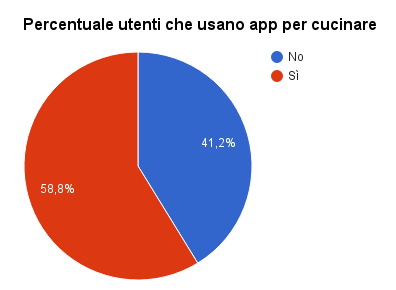
\includegraphics[scale=0.45]{img/chart_usi_app_cucina}
\end{minipage}
\hfill
\begin{minipage}{.49\textwidth}
	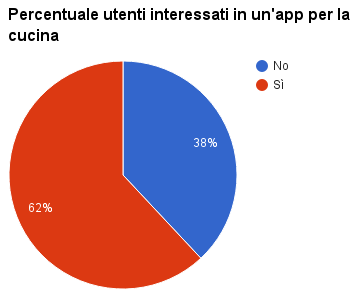
\includegraphics[scale=0.45]{img/chart_vorresti_app_cucina}
\end{minipage}
\end{figure}

\begin{quote}
	\textbf{Usi app o siti web per fare la spesa? Se hai risposto no, ti interesserebbe un'app per fare la spesa?}
\end{quote}

Come nel caso precedente, si vuole misurare l'utilizzo e l'interesse verso un'applicazione che aiuti gli utenti a fare
la spesa. Dai risultati emerge uno scarso utilizzo di applicazioni per fare la spesa, nonché un interesse molto meno marcato
che nel caso della domanda precedente.

\begin{figure}[H]
\centering
\begin{minipage}{.48\textwidth}
	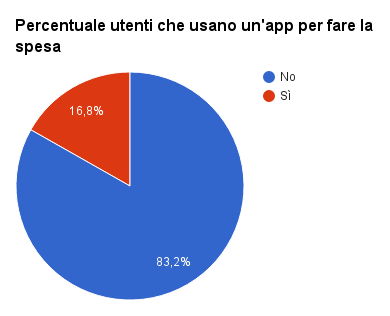
\includegraphics[scale=0.45]{img/chart_usi_app_spesa}
\end{minipage}
\hfill
\begin{minipage}{.49\textwidth}
	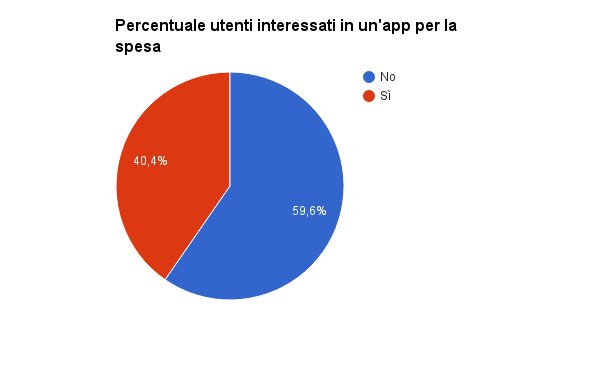
\includegraphics[scale=0.45]{img/chart_vorresti_app_spesa}
\end{minipage}
\end{figure}

\subsection{Analisi combinata dei dati}
Per ottenere ulteriori informazioni sugli utenti si sono considerati i
dati aggregati nel seguente modo:

\begin{quote}
	\textbf{Competenze digitali per fascia d'età}
\end{quote}
I dati sono stati combinati per ottenere maggiori informazioni a riguardo
l'utilizzo da parte degli utenti degli smartphone. Come era prevedibile,
la maggior parte dei giovani risulta essere competente con lo smartphone,
mentre le persone in età avanzata si attestano su valori relativamente
bassi. Le persone nelle fasce intermedie si sono dichiarate mediamente competenti
per quanto riguarda l'utilizzo di smartphone e computer.
\begin{figure}[H]
\centering
	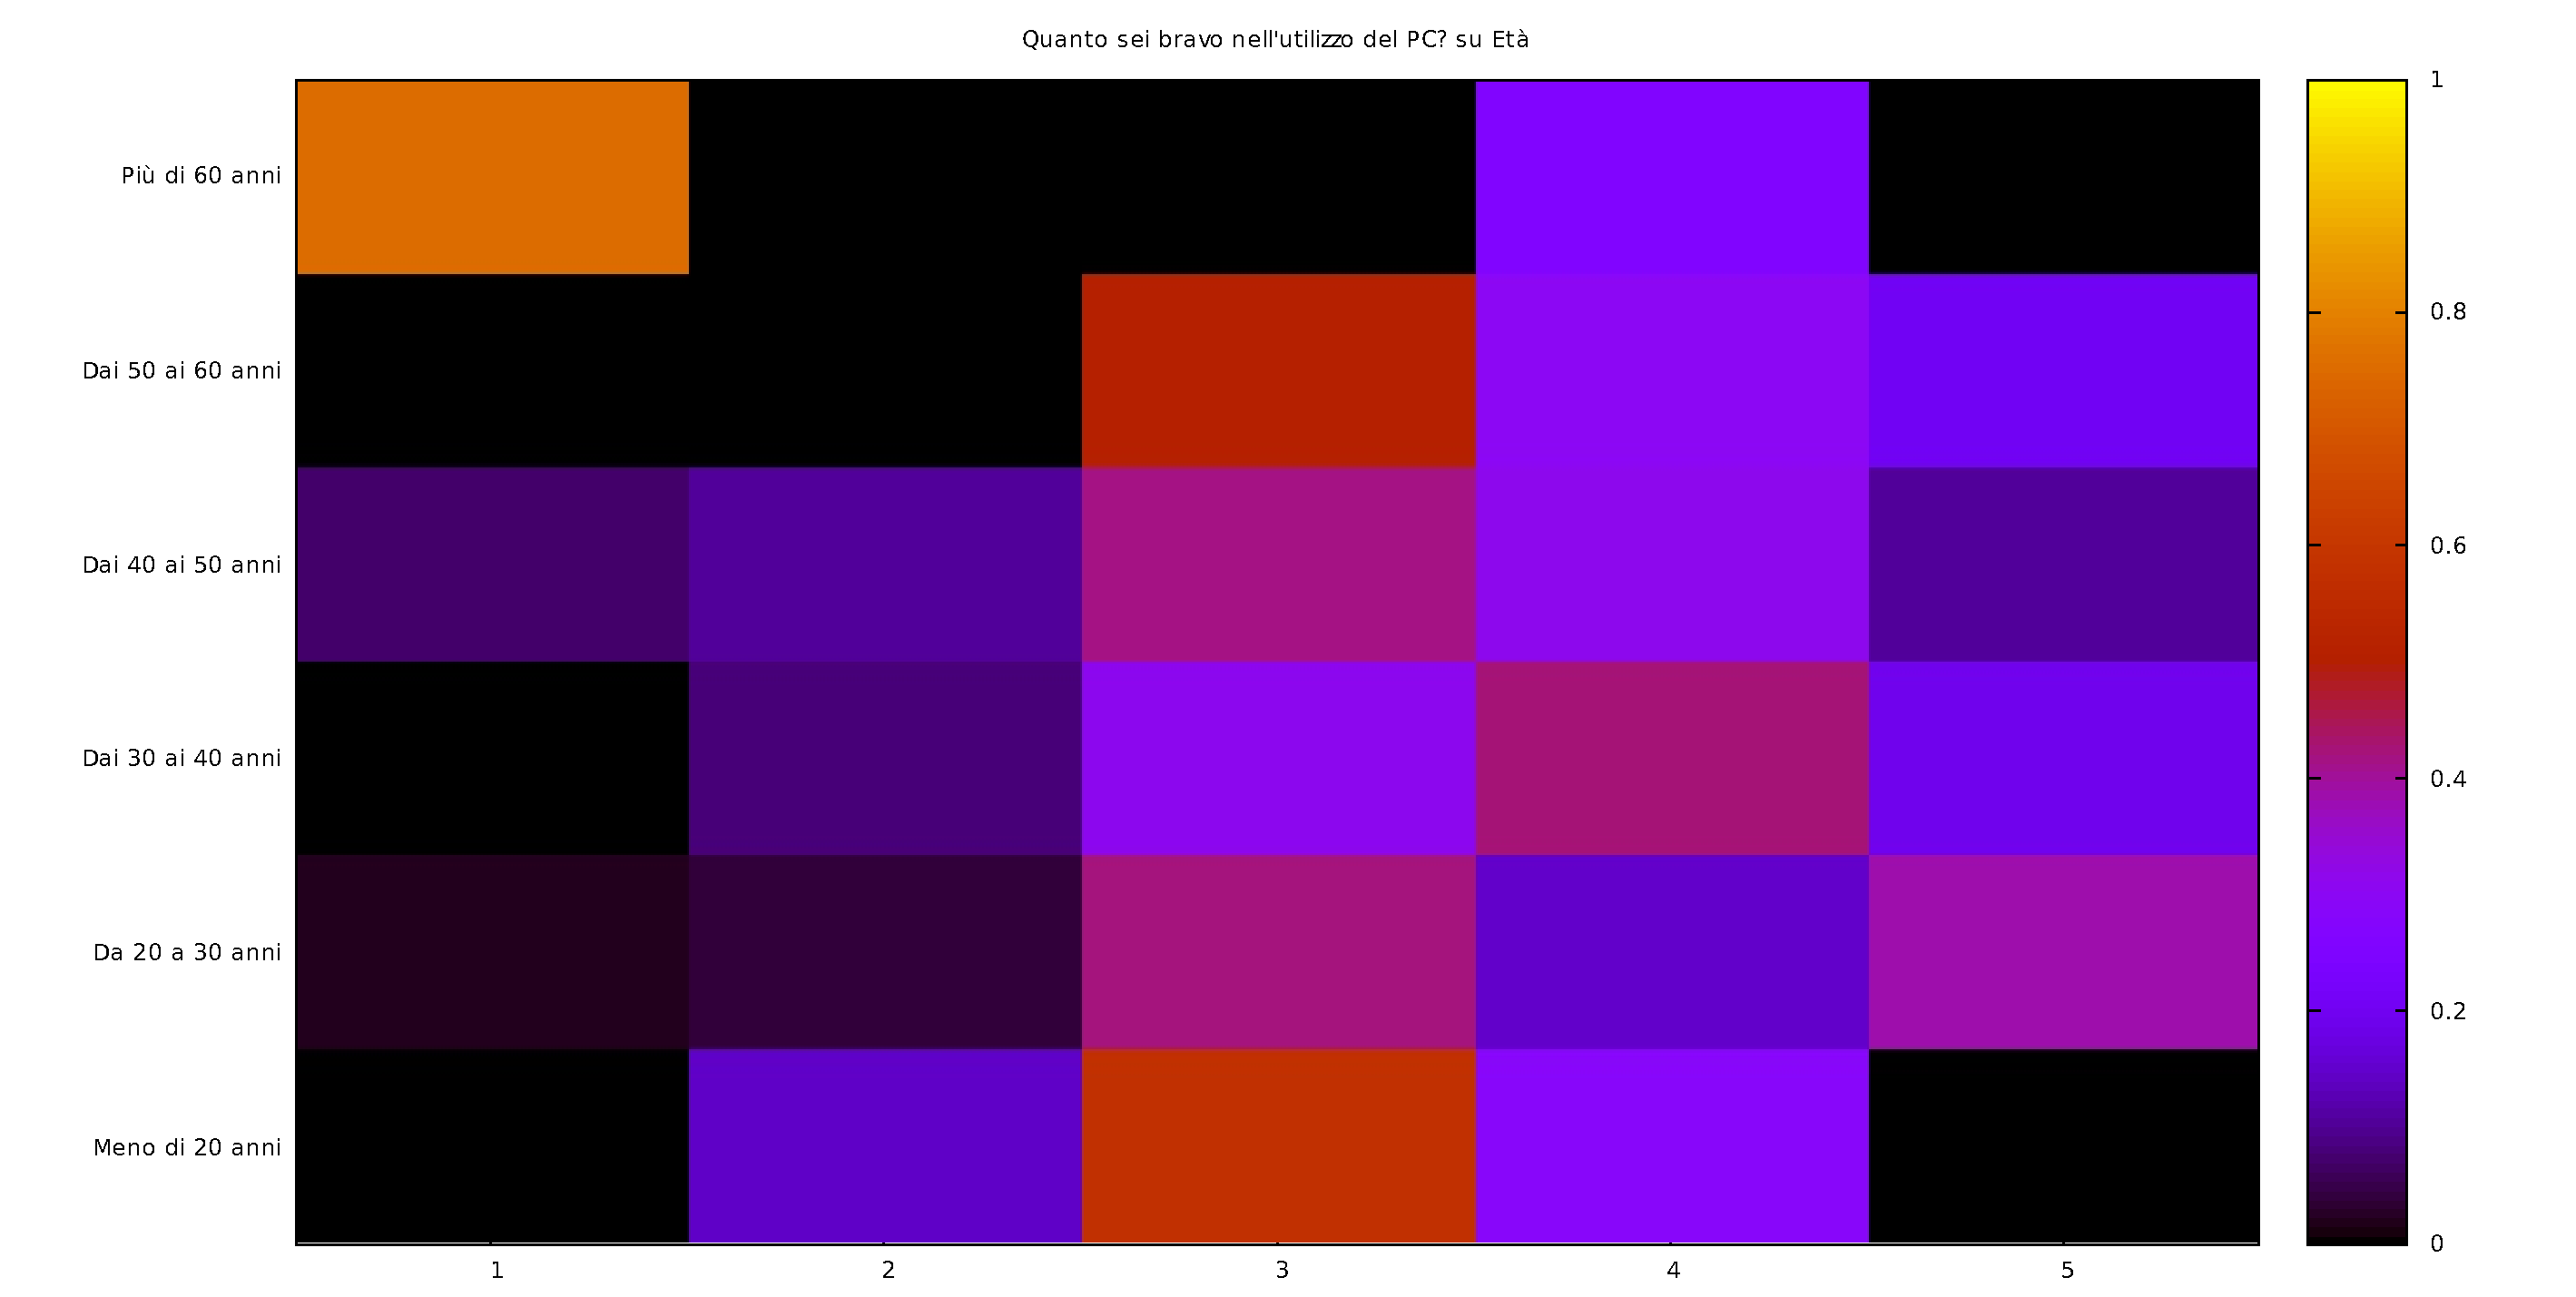
\includegraphics[width=\textwidth]{img/heatmap_pc_eta}
\end{figure}
\begin{figure}[H]
	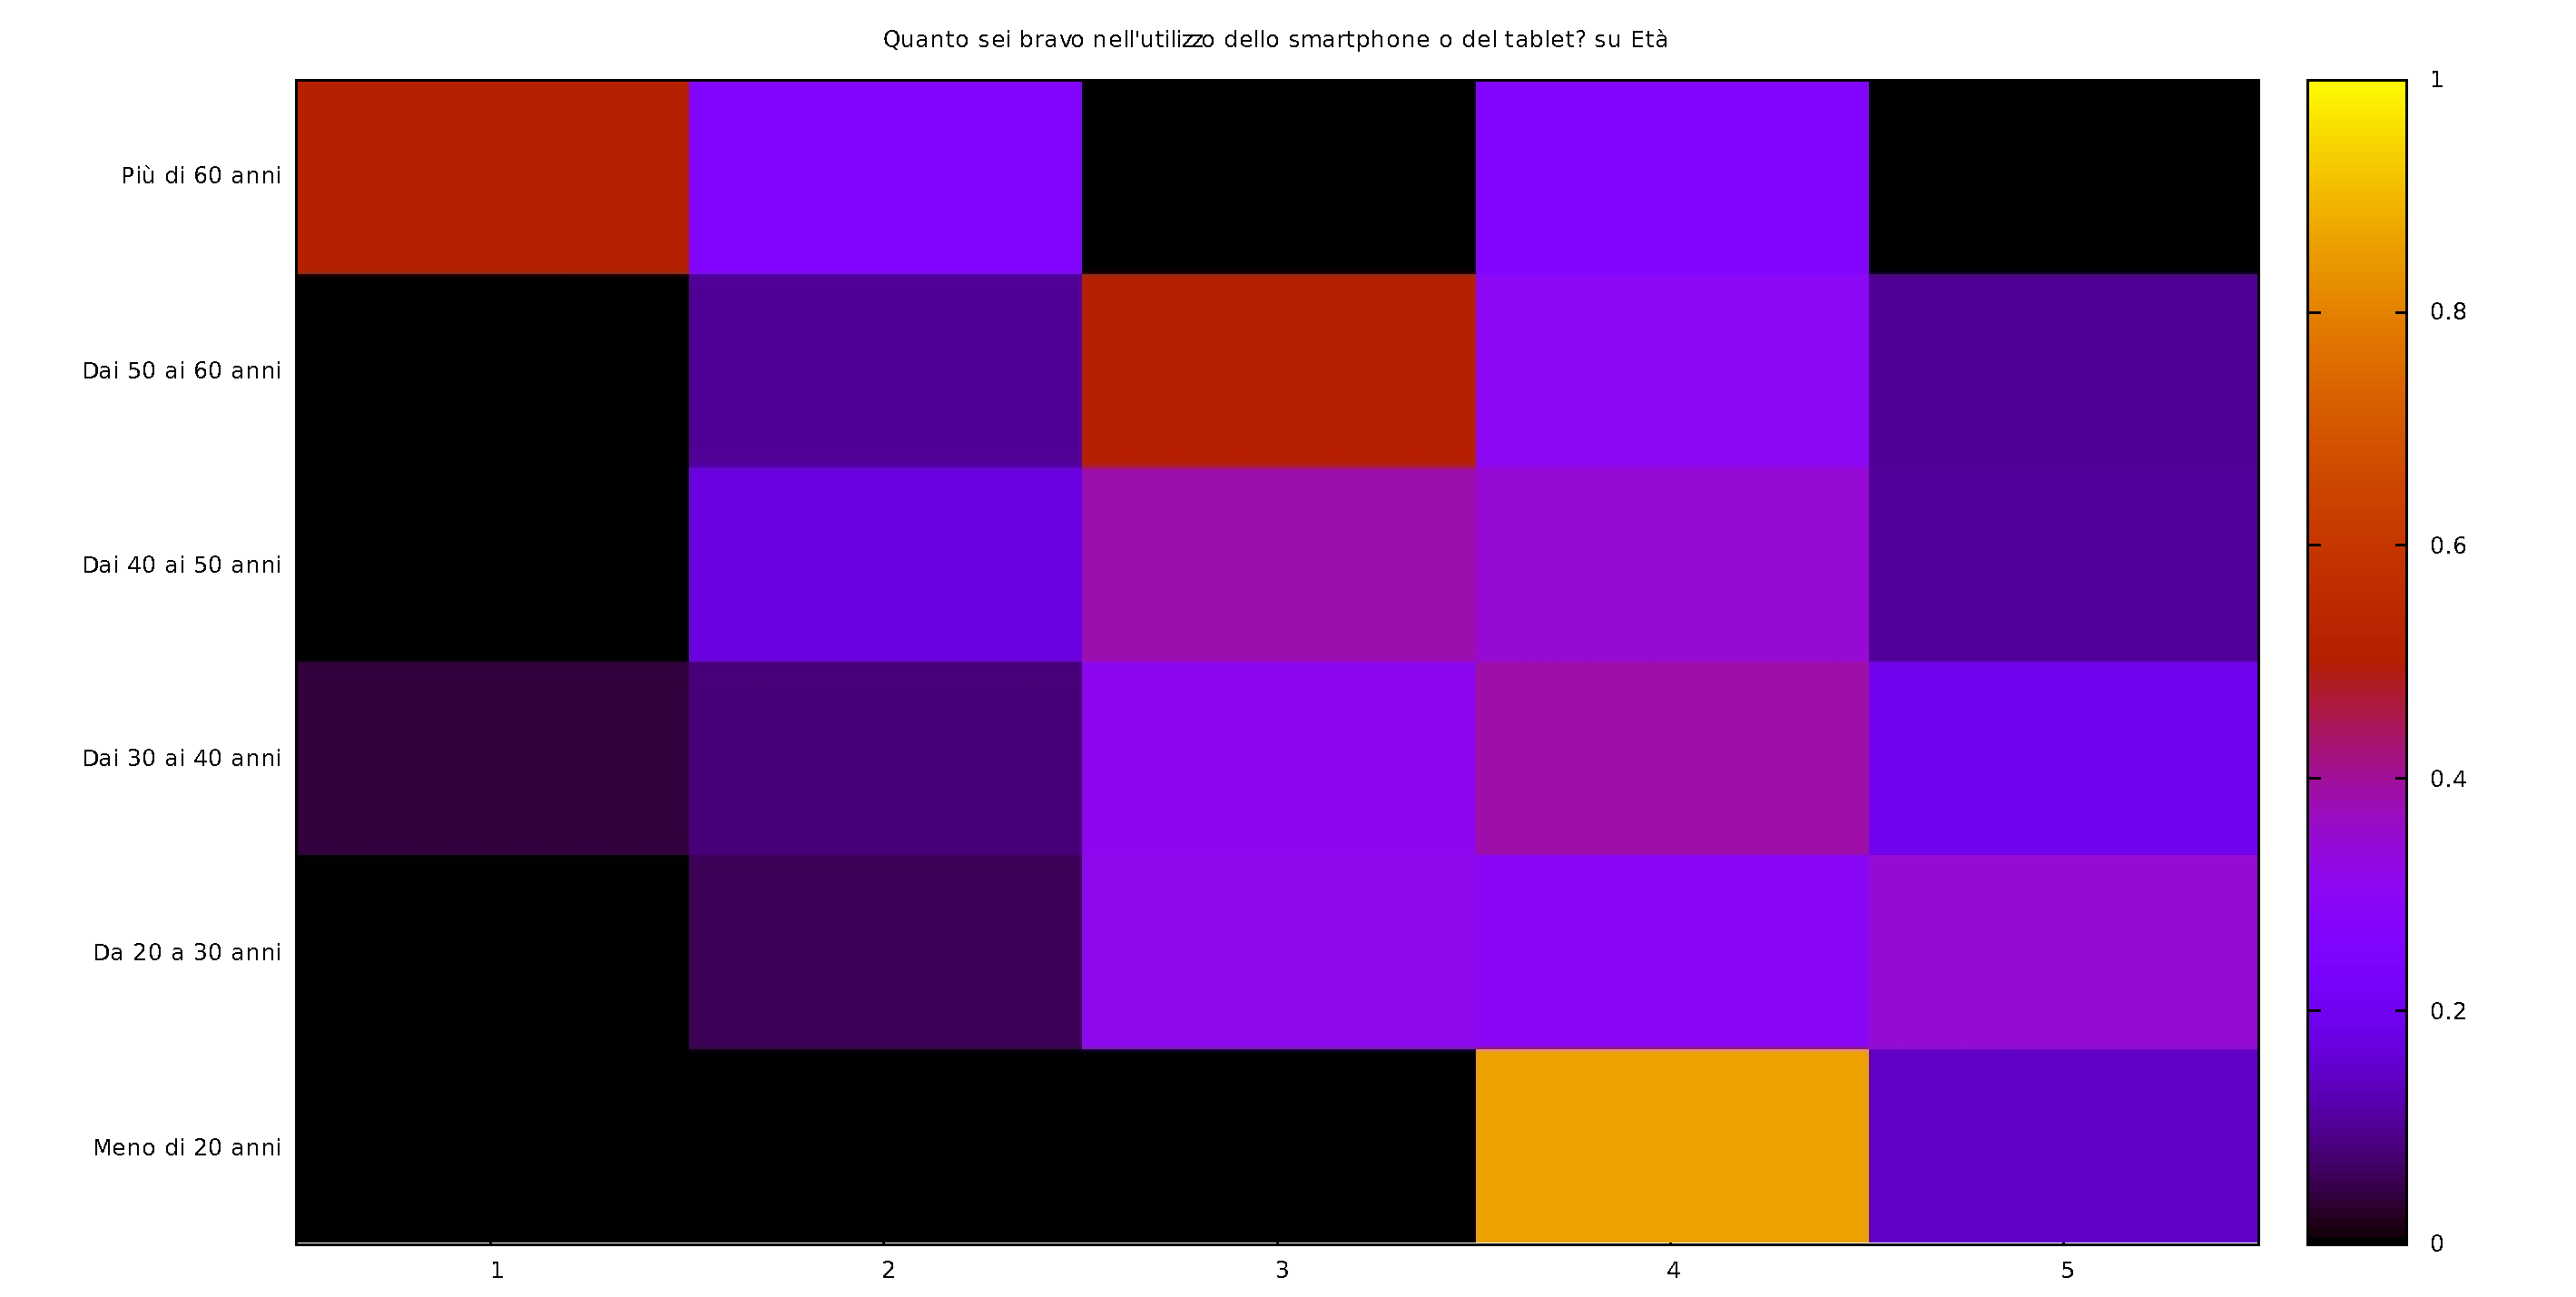
\includegraphics[width=\textwidth]{img/heatmap_smartphone_eta}
\end{figure}


\begin{quote}
	\textbf{Autovalutazione della bravura in cucina con o senza l'utilizzo
	di applicazioni}
\end{quote}

È stato inoltre valutato il rapporto fra la competenza culinaria e l'utilizzo di applicazioni 
di aiuto alla cucina. L'utilizzo di un'applicazione, contrariamente a quanto si potrebbe
anticipare, è più frequente fra chi si considera abile in cucina.

\begin{figure}[H]
	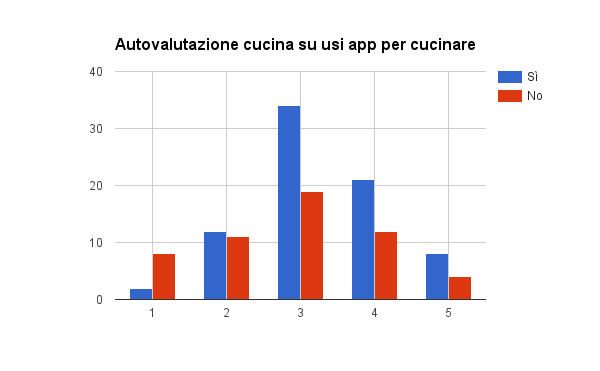
\includegraphics[width=\textwidth]{img/chart_autovalutazione_e_usi_app}
\end{figure}
